%% 9. OpenCL

\begin{frame}{History of OpenCL}

\begin{minipage}{0.7\textwidth}
\begin{block}{Prior to 2008}
  \begin{itemize}
   \item OpenCL developed by Apple Inc.
  \end{itemize}
\end{block}

\begin{block}{2008}
  \begin{itemize}
   \item OpenCL working group formed at Khronos Group
   \item OpenCL specification 1.0 released
  \end{itemize}
\end{block}

\begin{block}{2010}
  \begin{itemize}
   \item OpenCL 1.1 (multi-device, subbuffer manipulation)
  \end{itemize}
\end{block}

\begin{block}{2011}
  \begin{itemize}
   \item OpenCL 1.2 (device partitioning)
  \end{itemize}
\end{block}

\begin{block}{2013}
  \begin{itemize}
   \item OpenCL 2.0 (shared virtual memory, SPIR, etc.)
  \end{itemize}
\end{block}

\end{minipage} \hfill
\begin{minipage}{0.25\textwidth}
 
\includegraphics[width=0.99\textwidth]{figures/opencl.jpg}
 
 \vspace*{5cm}
\end{minipage}


\end{frame}


\begin{frame}{OpenCL}

\begin{block}{Similar to CUDA}
  \begin{itemize}
   \item Kernel language is a subset of C
   \item Explicit memory management, host-device transfers
   \item Memory model: local, shared, global
  \end{itemize}
\end{block}


\begin{block}{Different from CUDA}
  \begin{itemize}
   \item Support by many vendors
   \item No compiler-wrapper, only a shared library
   \item Kernel compilation usually at runtime
  \end{itemize}
\end{block}

\end{frame}

%%%%%%%%%%%%%%

% \begin{frame}{OpenCL Platform Model}
%  \begin{center}
%    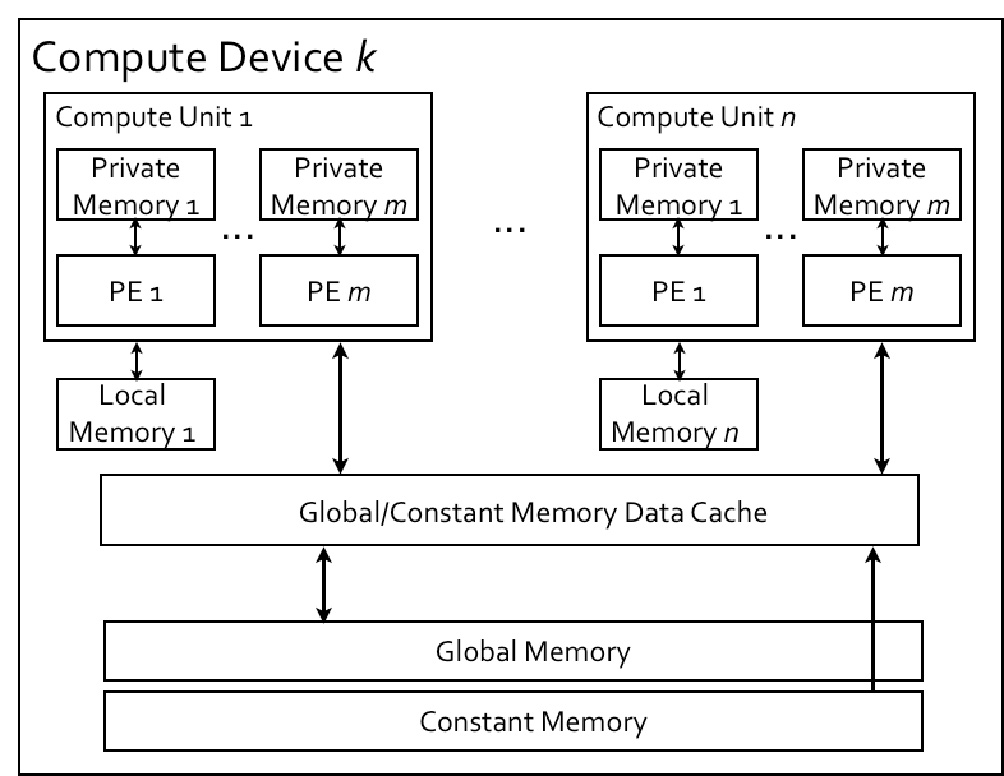
\includegraphics[width=0.80\textwidth]{figures/opencl-device}
%  \end{center}
% \end{frame}

%%%%%%%%%%%%%%%%%%%% Platform Model %%%%%%%%%%%%%%%%%%%%%%

% \begin{frame}{OpenCL Platform Model}
%  \begin{center}
%    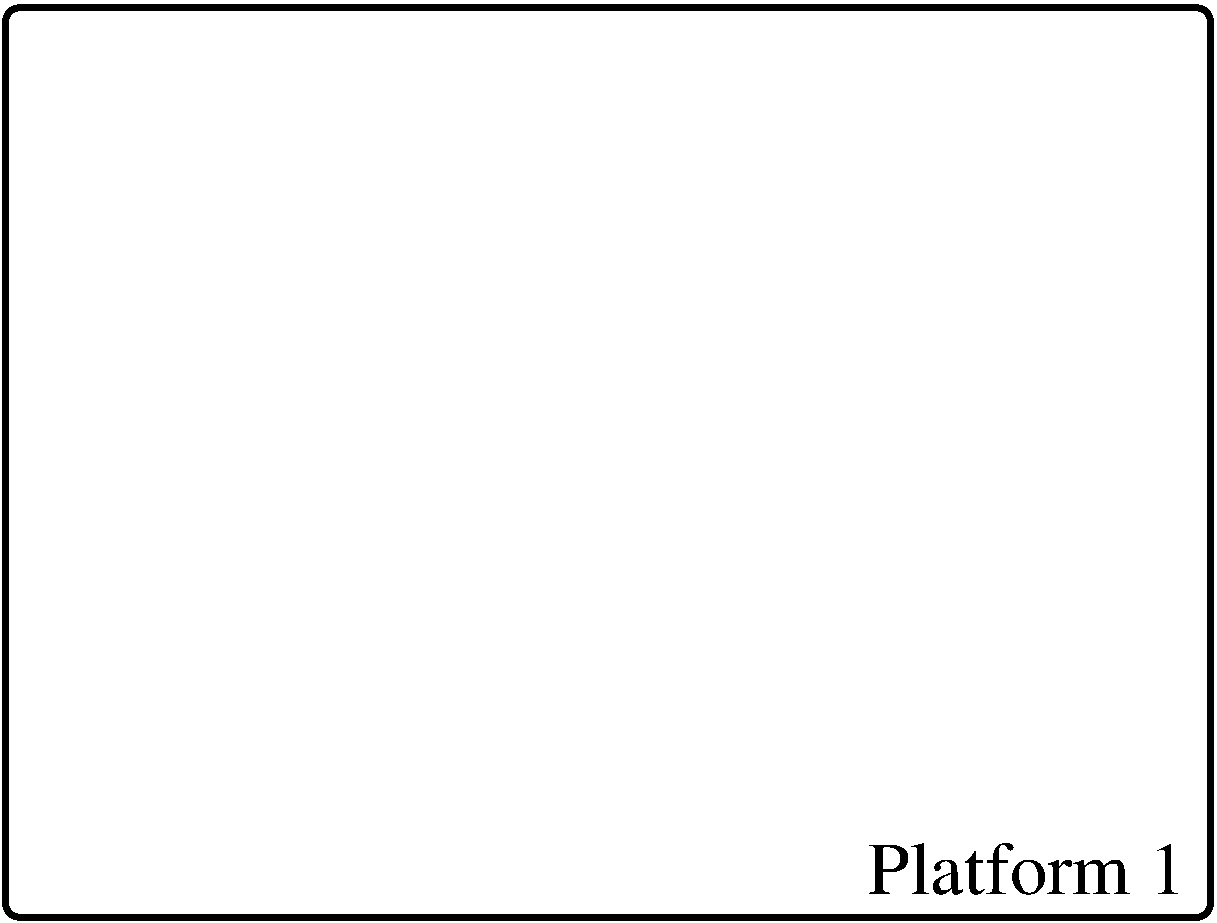
\includegraphics[width=0.80\textwidth]{figures/opencl-2.pdf}
%  \end{center}
% \end{frame}
% 
% \begin{frame}{OpenCL Platform Model}
%  \begin{center}
%    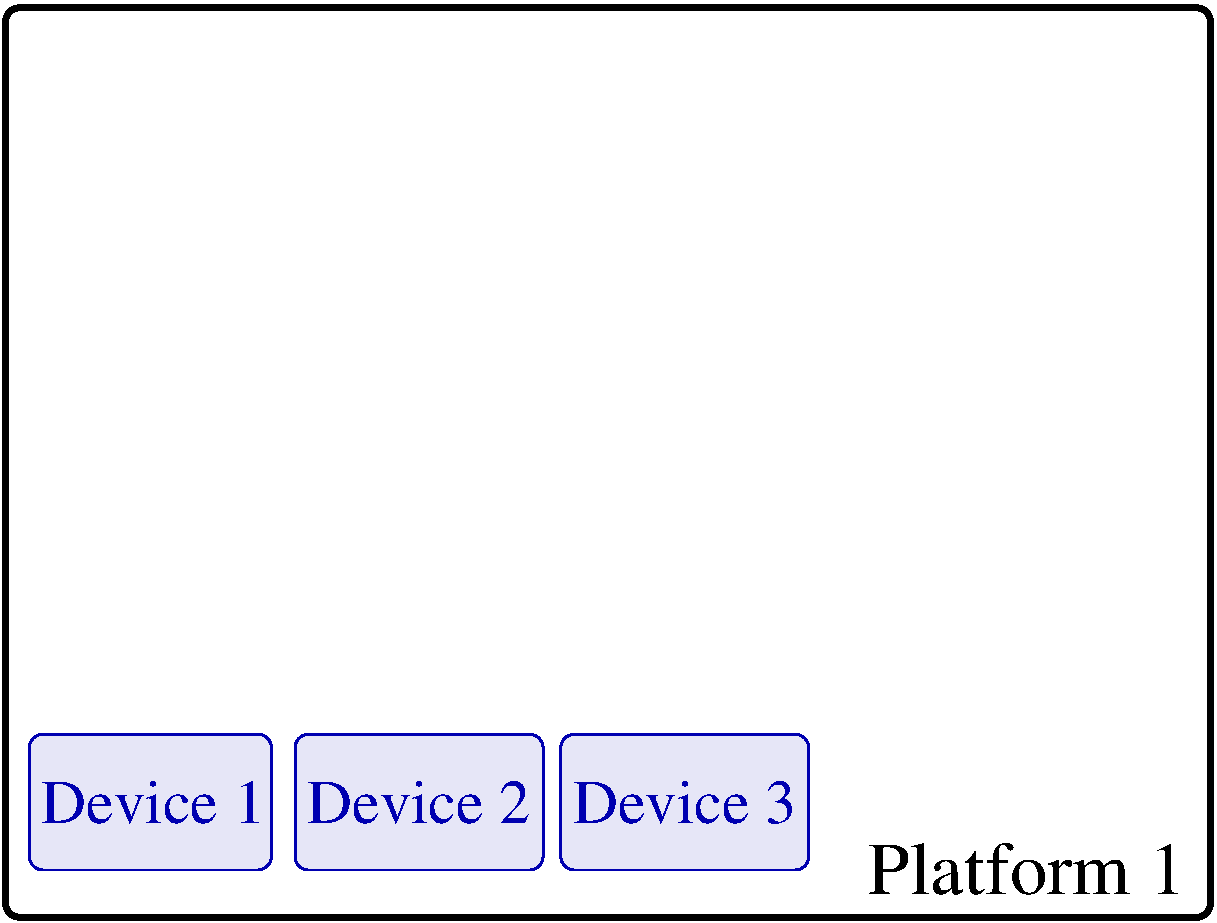
\includegraphics[width=0.80\textwidth]{figures/opencl-3.pdf}
%  \end{center}
% \end{frame}
% 
% \begin{frame}{OpenCL Platform Model}
%  \begin{center}
%    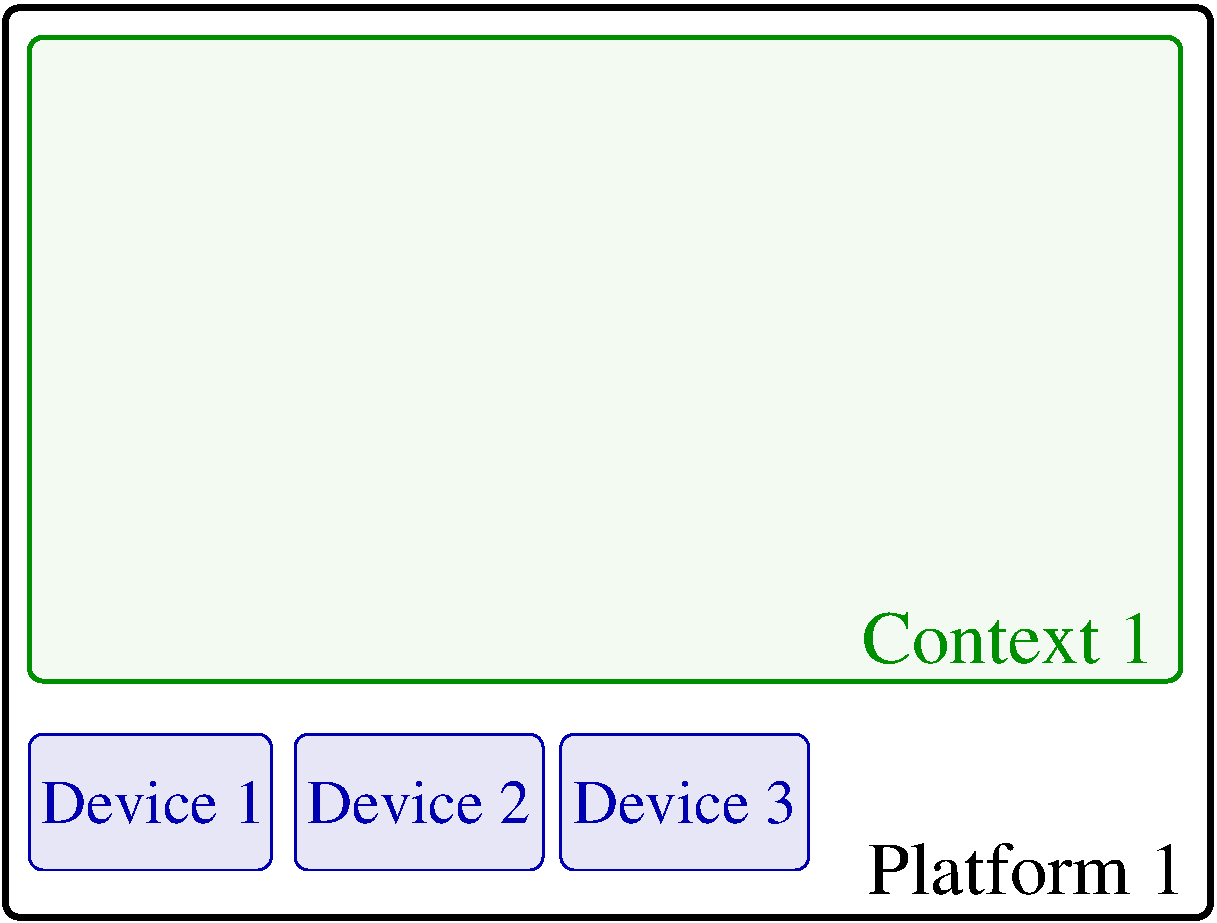
\includegraphics[width=0.80\textwidth]{figures/opencl-4.pdf}
%  \end{center}
% \end{frame}
% 
% \begin{frame}{OpenCL Platform Model}
%  \begin{center}
%    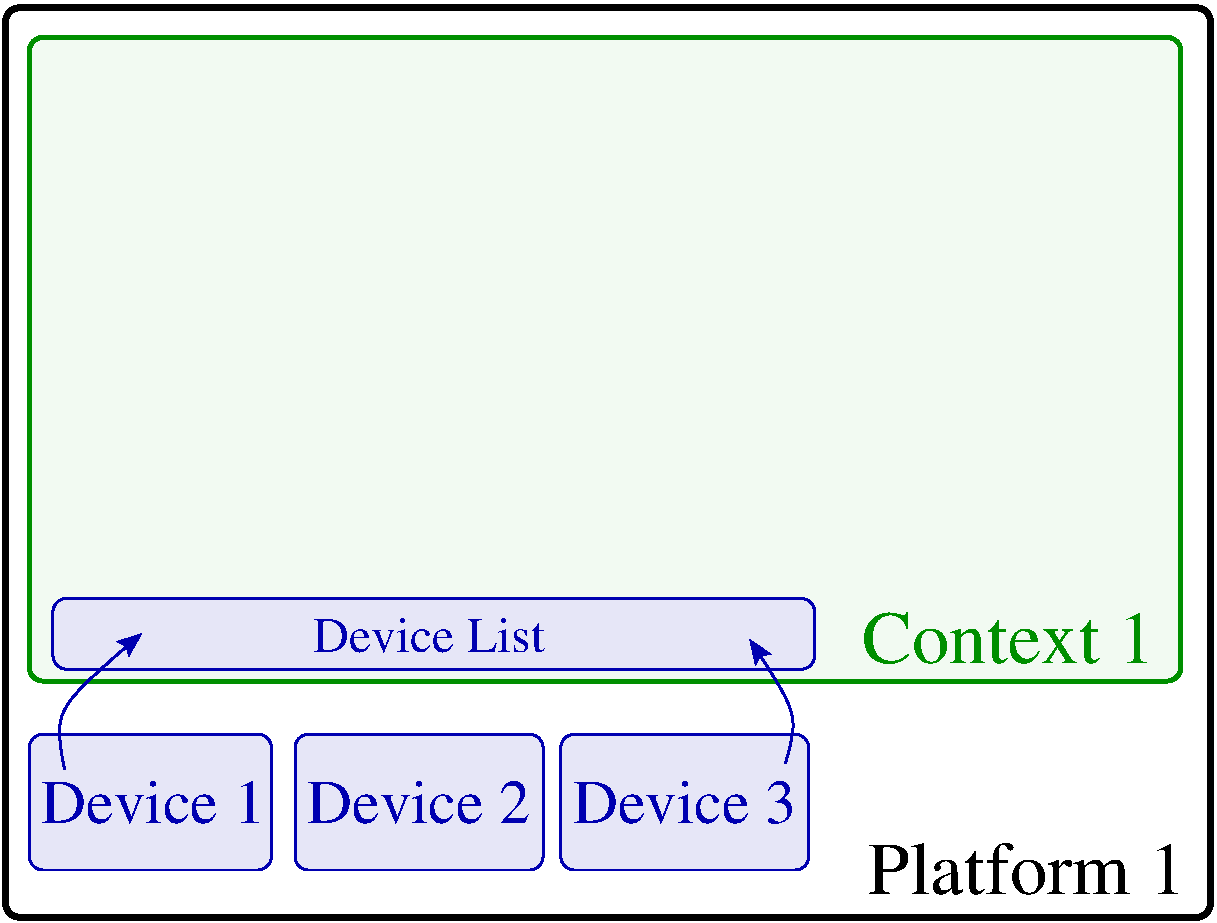
\includegraphics[width=0.80\textwidth]{figures/opencl-5.pdf}
%  \end{center}
% \end{frame}
% 
% \begin{frame}{OpenCL Platform Model}
%  \begin{center}
%    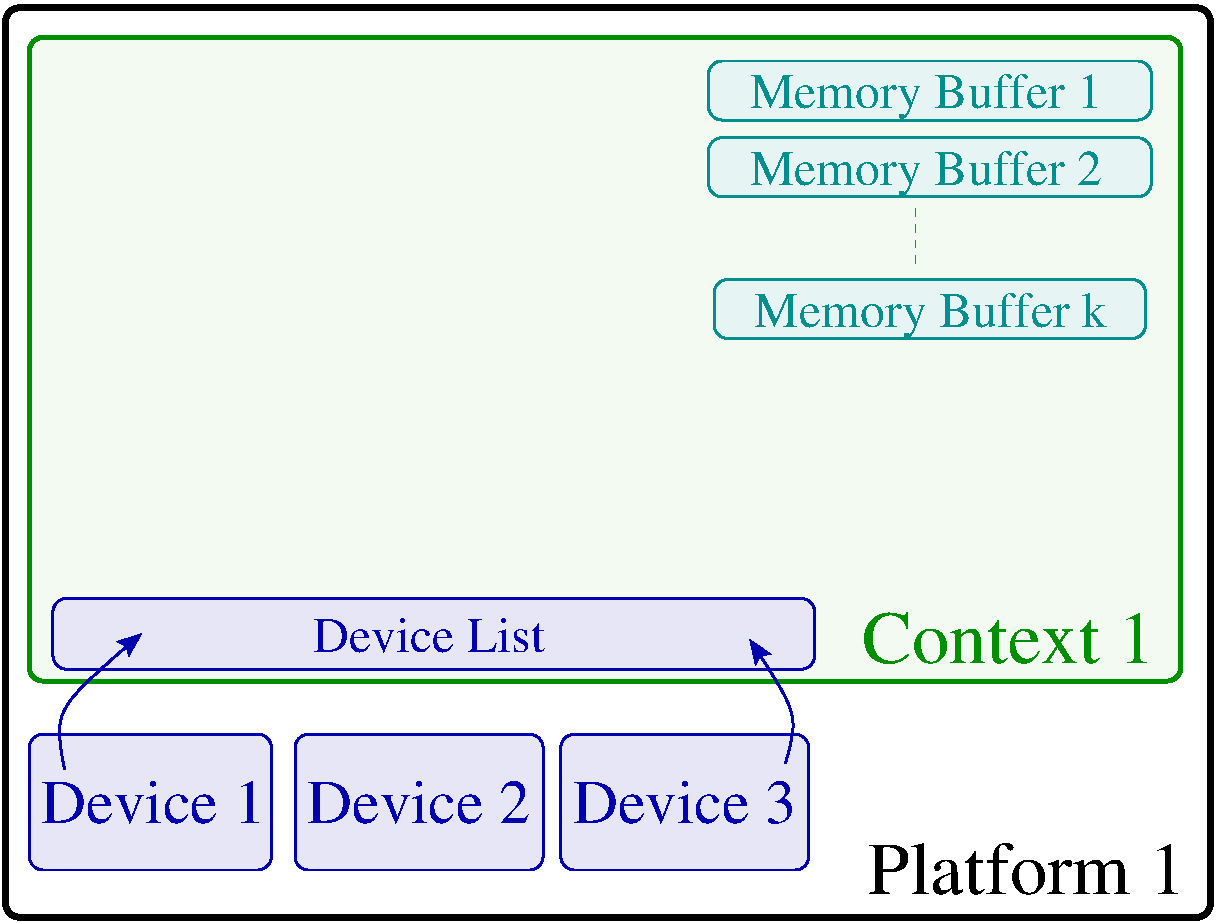
\includegraphics[width=0.80\textwidth]{figures/opencl-6.pdf}
%  \end{center}
% \end{frame}
% 
% \begin{frame}{OpenCL Platform Model}
%  \begin{center}
%    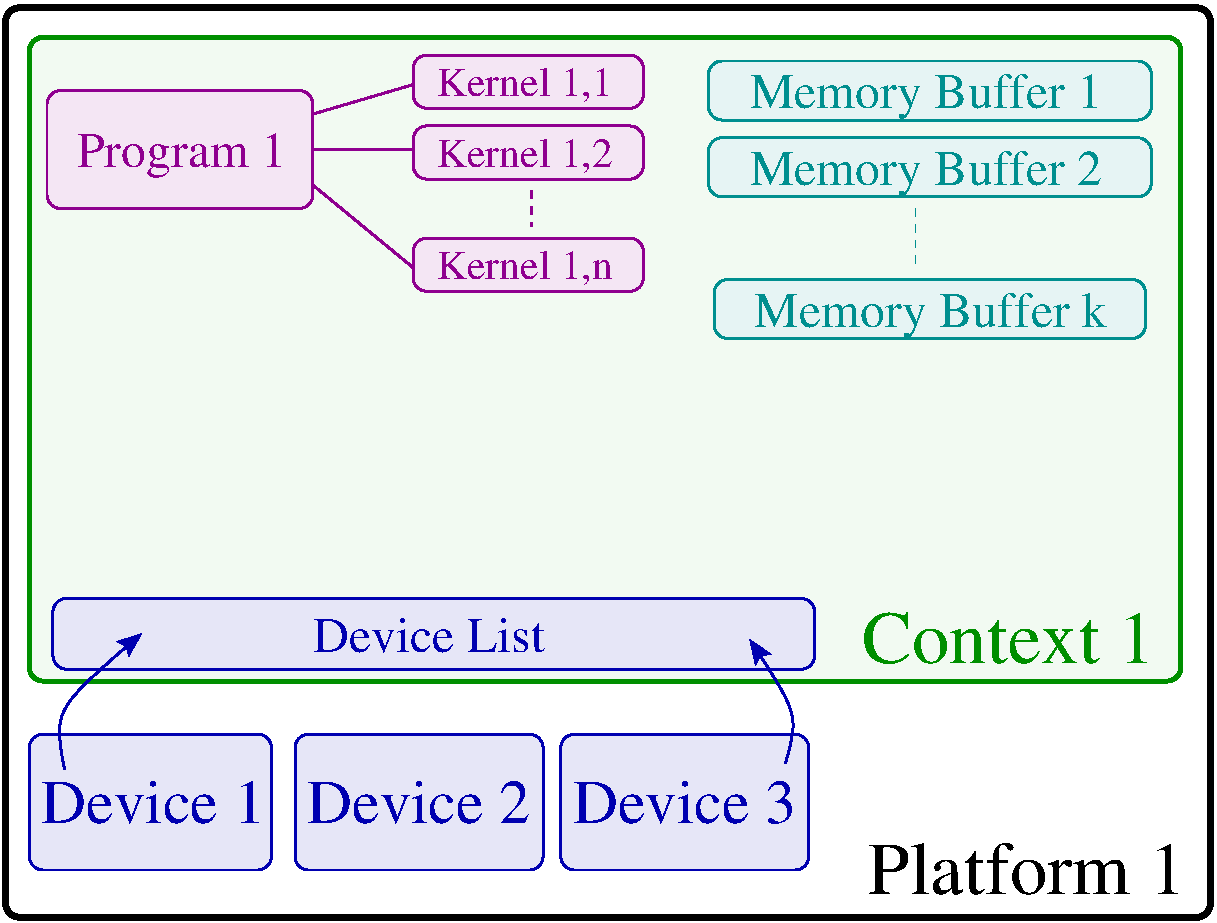
\includegraphics[width=0.80\textwidth]{figures/opencl-7.pdf}
%  \end{center}
% \end{frame}
% 
% \begin{frame}{OpenCL Platform Model}
%  \begin{center}
%    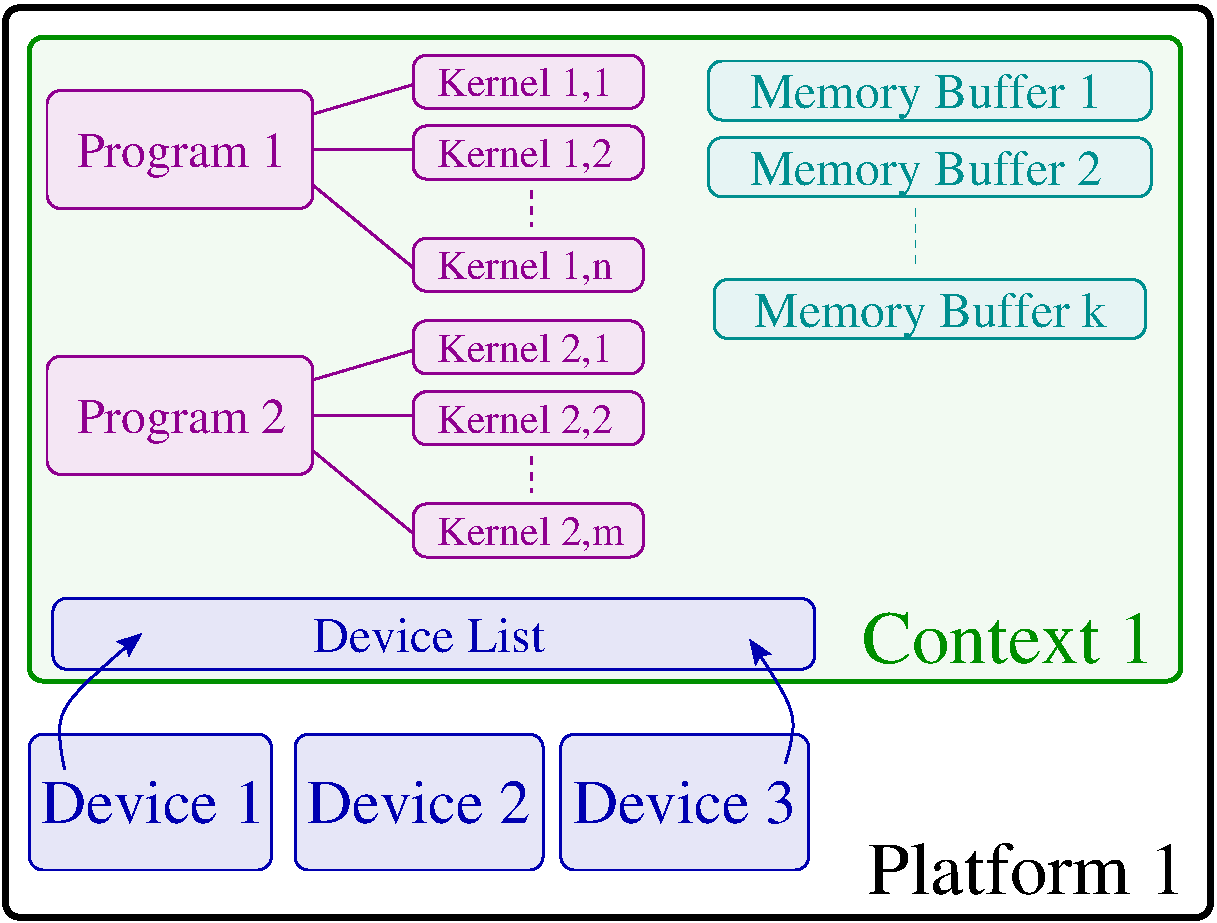
\includegraphics[width=0.80\textwidth]{figures/opencl-8.pdf}
%  \end{center}
% \end{frame}

\begin{frame}{OpenCL Platform Model}
 \begin{center}
   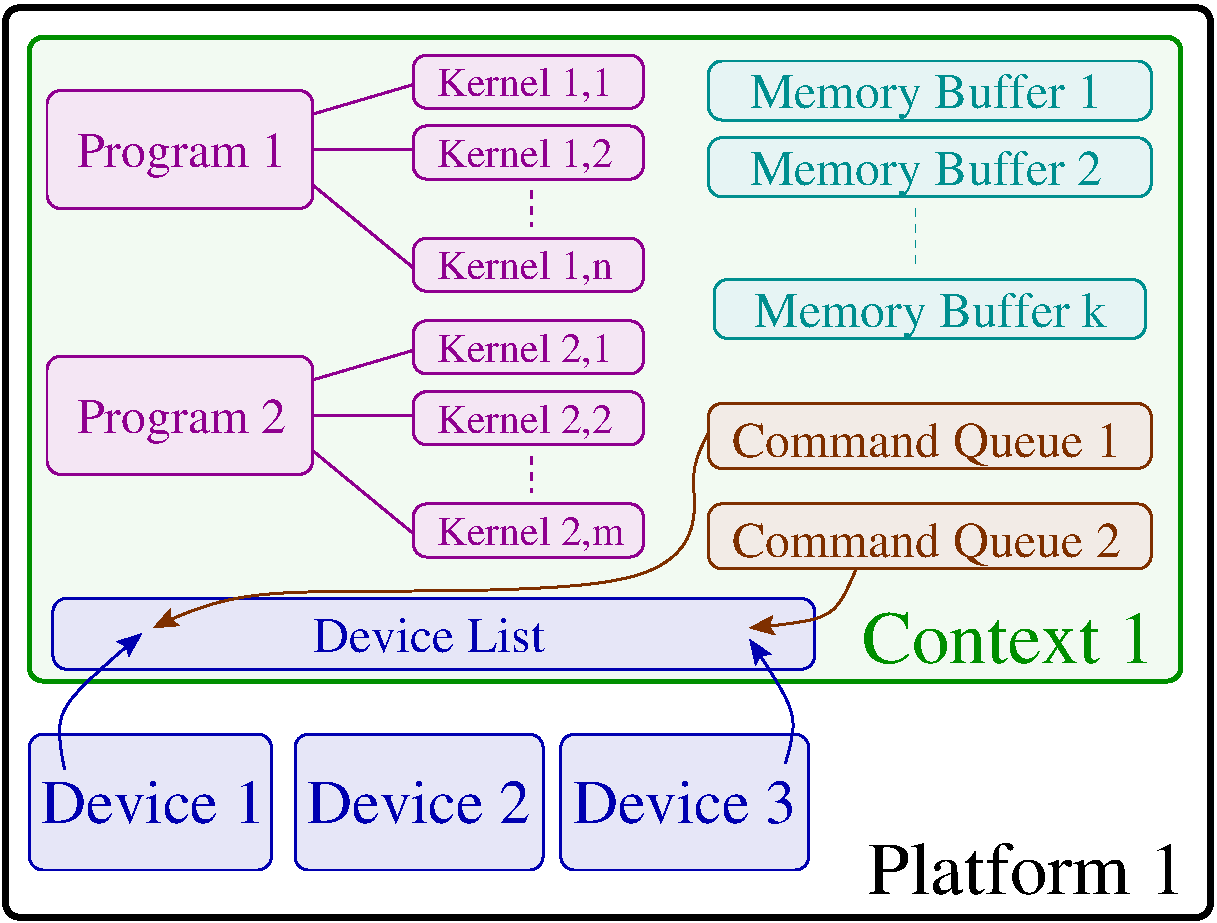
\includegraphics[width=0.80\textwidth]{figures/opencl-full.pdf}
 \end{center}
\end{frame}


% Explain differences to CUDA

\begin{frame}{OpenCL}

\begin{minipage}{0.7\textwidth}
\begin{block}{OpenCL Thread Control (1D) vs. CUDA}
 \begin{itemize}
  \item Local ID in block: \lstinline|get_local_id(0)|
  \item Threads per block: \lstinline|get_local_size(0)|
  \item ID of block: \lstinline|get_group_id()|
  \item No. of blocks: \lstinline|get_num_groups()|
  \item Global thread ID: \lstinline|get_global_id()|
  \item No. of threads: \lstinline|get_global_size()|
 \end{itemize}
\end{block}
\end{minipage}
\begin{minipage}{0.25\textwidth}
\begin{block}{}
 \begin{itemize}
  \item {\color{darkgreen}\lstinline|threadIdx.x|}
  \item {\color{darkgreen}\lstinline|blockDim.x|}
  \item {\color{darkgreen}\lstinline|blockIdx.x|}
  \item {\color{darkgreen}\lstinline|gridDim.x|}
  \item
 \end{itemize}
\end{block}
\vspace*{0.1cm}
\end{minipage}

\end{frame}
